\section{Applications}

The relation between $\deg(D)$ and $l(D)$ for a curve of genus $g$ can be partially determined by the Riemann-Roch theorem (\Cref{thm:rr}). $l(D)$ of a divisor of negative degree is 0 by \Cref{corollary:ldzero}. For divisors $D$ with $\deg(D)>2g-2$, one gets $l(D)=\deg(D)-g+1$ since $l(\kappa-D)=0$ again by \Cref{corollary:ldzero}. For each additional point added to $D$, $l(D)$ either stays the same or increases by 1 by \Cref{lemma:ldp}. So, the graph of $\deg(D)$ versus $l(D)$ in $\mathbb{Z}\times\mathbb{Z}$ would look like \Cref{fig:degdld}, where the gray region represents the possibilities.

This application is from Chapter 7 in \cite{ref:keith} (Keith).

\begin{figure}
    \centering
    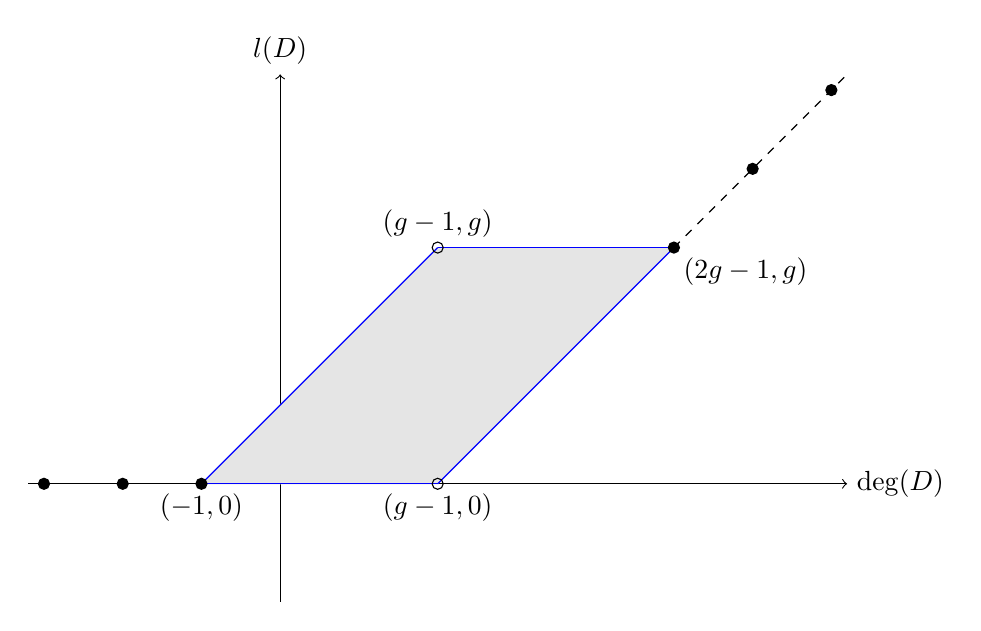
\begin{tikzpicture}
        \draw[->] (-3.2, 0) -- (7.2, 0) node[right] {$\deg(D)$};
        \draw[->] (0, -1.5) -- (0, 5.2) node[above] {$l(D)$};
        \filldraw[gray!20] (-1,0) -- (2,0) -- (5,3) -- (2,3) -- (-1,0);
        \draw[scale=1.0, domain=2:5, smooth, variable=\x, blue] plot ({\x}, {\x-2});
        \draw[scale=1.0, domain=-1:2, smooth, variable=\x, blue] plot ({\x}, {\x+1});
        \draw[scale=1.0, domain=2:5, smooth, variable=\x, blue] plot ({\x}, {3});
        \draw[scale=1.0, domain=-1:2, smooth, variable=\x, blue] plot ({\x}, {0});
        \filldraw[black] (-1,0) circle (2pt) node[anchor=north]{$(-1,0)$};
        \filldraw[black] (-2,0) circle (2pt) node[anchor=west]{};
        \filldraw[black] (-3,0) circle (2pt) node[anchor=west]{};
        \filldraw[black] (5,3) circle (2pt) node[anchor=north west]{$(2g-1,g)$};
        \filldraw[black] (6,4) circle (2pt) node[anchor=west]{};
        \filldraw[black] (7,5) circle (2pt) node[anchor=west]{};
        \draw[] (2,0) circle (2pt) node[anchor=north]{$(g-1,0)$};
        \draw[] (2,3) circle (2pt) node[anchor=south]{$(g-1,g)$};
        \draw[dashed] (5,3) -- (7.2,5.2);
    \end{tikzpicture}
    \caption{Graph of $\deg(D)$ versus $l(D)$ for a curve with genus $g$}
    \label{fig:degdld}
\end{figure}

\begin{theorem}[Group Structure of Curves]\label{thm:group}
    Let $\curveC$ be a non-singular projective curve of degree $3$ in $\projective_2$. Let $O$ be an inflection point of $\curveC$. There is a unique additive group structure on $\curveC$ such that $O$ is the zero element and for any $P,Q,R\in\curveC$,
    $$P+Q+R=0$$
    if and only if $P$, $Q$, $R$ are the three points of intersection of a line with $\curveC$.
\end{theorem}

Proof of \Cref{thm:group} is from Theorem 6.39 in \cite{ref:kirwan} (Kirwan).

\begin{proof}
    $-O=O$ and for $P\neq O$, $-P$ is the other intersection of the line through $P$ and $O$. And $P+Q=-R$ where $R$ is the other intersection of the line through $P$ and $Q$. Therefore, if there is a structure, it is unique. Commutativity is inherent from the definition of the operation.
    
    For the associativity, let
    \begin{align*}
        A &= P+Q\\
        B &= A+R\\
        C &= Q+R\\
        D &= P+C
    \end{align*}
    and show that $B=D$. There is a linear polynomial that vanishes at $P$, $Q$, $-A$. The ratio of this polynomial to the polynomial that vanishes at $A$, $-A$, $O$ defines a meromorphic function $\phi_A$ with zeroes at $P$, $Q$ and poles at $A$, $O$. Similarly, $\phi_B$ can be obtained with zeroes at $A$, $R$ and poles at $B$, $O$. Then, $\phi_A\phi_B$ is a meromorphic function with zeroes at $P$, $Q$, $R$ and poles at $B$, $O$, $O$. Doing this for $C$ and $D$, one obtains a meromorphic function $\phi_C\phi_D$ with zeroes at $P$, $Q$, $R$ and poles at $D$, $O$, $O$. The ratio of $\phi_C\phi_D$ and $\phi_A\phi_B$ has a simple zero at $D$ and a simple pole at $B$. By the Riemann-Roch theorem  (\Cref{thm:rr}),
    $$l(B)-l(\kappa-B)=\deg(B)-g+1$$
    $l(\kappa-B)=0$ since $\deg(\kappa-B)=\deg(\kappa)-\deg(B)=-1<0$. So, $l(B)=1$. That is, the only meromorphic functions on $\curveC$ with at most a simple pole at $B$ are the constant functions. Therefore, $B=D$.
\end{proof}

\begin{figure}
    \centering
    \begin{tikzpicture}[scale=1.7]
        \draw[->] (-2.3, 0) -- (3.4, 0) node[right] {$x$};
        \draw[->] (0, -3.0) -- (0, 3.0) node[above] {$y$};
        \draw[domain=-1.987076:3.1,samples=100,smooth,variable=\x,blue] plot ({\x},{sqrt((\x^3)/3.375 - (\x)/1.5 + 1)});
        \draw[domain=-1.987076:3.1,samples=100,smooth,variable=\x,blue] plot ({\x},{-sqrt((\x^3)/3.375 - (\x)/1.5 + 1)});
        \node (P) at (-1.95, 0.321) {};
        \node (Q) at (0.6, 0.81486) {};
        \node (R) at (0.16233, -0.945) {};
        \node (NPR) at (3.0, -2.64575) {};
        \node (PR) at (3.0, 2.64575) {};
        \node (NPQ) at (1.47657, 0.98463) {};
        \node (PQ) at (1.47657, -0.98463) {};
        \node (NPQR) at (-1.63584, -0.8908) {};
        \filldraw[black] (P) circle (1pt) node[anchor=east]{$P$};
        \filldraw[black] (Q) circle (1pt) node[anchor=south]{$Q$};
        \filldraw[black] (R) circle (1pt) node[anchor=north]{$R$};
        \filldraw[black] (NPR) circle (1pt) node[anchor=west]{$-(P+R)$};
        \filldraw[black] (PR) circle (1pt) node[anchor=west]{$P+R$};
        \filldraw[black] (NPQ) circle (1pt) node[anchor=west]{$-(P+Q)$};
        \filldraw[black] (PQ) circle (1pt) node[anchor=west]{$P+Q$};
        \filldraw[black] (NPQR) circle (1pt) node[anchor=east]{$-(P+Q+R)$};
        \draw[dashed] (P) -- (NPQ);
        \draw[dashed] (P) -- (NPR);
        \draw[dashed, color=orange] (NPQ) -- (PQ);
        \draw[dashed, color=orange] (NPR) -- (PR);
        \draw[dashed] (NPQR) -- (PQ);
        \draw[dashed] (NPQR) -- (PR);
    \end{tikzpicture}
    \caption{Associativity of the elliptic curve group operation}
    \label{fig:ec}
\end{figure}

\begin{remark}
    \Cref{thm:group}, for a finite field instead of $\CC$, is what makes elliptic curve cryptography possible, which is an integral part of the modern cryptology.
\end{remark}

